\documentclass[a4paper]{scrartcl}
\usepackage[utf8]{inputenc}
\usepackage[T1]{fontenc}
\usepackage{fancyhdr}
\usepackage{hyperref}
\usepackage{graphicx}
\usepackage[swedish]{babel}
\usepackage[center]{caption}
\usepackage[table]{xcolor}
\usepackage{epstopdf}
\usepackage{hyperref}
\usepackage{listings}
\usepackage[table]{xcolor}
\usepackage{fixltx2e}
\usepackage{listings}
\usepackage{float}
\usepackage{tabularx}

\hypersetup{
    pdfborder = {0 0 0}
}

% kod
\definecolor{dkgreen}{rgb}{0,0.6,0}
\definecolor{gray}{rgb}{0.5,0.5,0.5}
\definecolor{mauve}{rgb}{0.58,0,0.82}
\lstset{
	language=VHDL,
	tabsize=4,
	columns=fullflexible,
	basicstyle=\footnotesize\ttfamily,
	%basicstyle=\footnotesize,
	keepspaces=true,
	keywordstyle=\color{blue},          % keyword style
	commentstyle=\color{dkgreen},       % comment style
	stringstyle=\color{mauve},         % string literal style
}


% Justera avstånd mellan rader i innehållsförteckningen
\usepackage{tocloft}

%  Automata
\usepackage{tikz}
\usetikzlibrary{arrows,automata}

\setlength\cftparskip{0pt}
\setlength\cftbeforesecskip{2pt}
\setlength\cftaftertoctitleskip{1cm}

%-----
% Fin header
\pagestyle{fancy}
\fancyhead[L]{\sffamily\leftmark}
\fancyhead[R]{\sffamily\rightmark}

\definecolor{light-gray}{gray}{0.95}

\let\oldtabularx\tabularx
\let\endoldtabularx\endtabularx
\renewenvironment{tabularx}{\rowcolors{2}{white}{light-gray}\oldtabularx}{\endoldtabularx}


\begin{document}

\newcommand{\signal}[1] {\texttt{#1}}
\newcommand{\state}[1] {\textbf{#1}}
\newcommand{\ohm} {$\Omega$}
\newcommand{\us} {$\mathrm{\mu s}$}
\newcommand{\tos} {$\rightarrow$}
\newcommand {\high} {\signal{'1'}}
\newcommand {\low} {\signal{'0'}}
\newcommand {\Tx} {T\textsubscript{x}}
\newcommand {\Rx} {R\textsubscript{x}}
\newcommand {\fullref}[1] {\ref{#1} \nameref{#1}}
\newcommand{\degcel}{\ensuremath{^\circ\mathrm{C}}}


%-----------------------------------------------------------

\begin{titlepage}
\centering
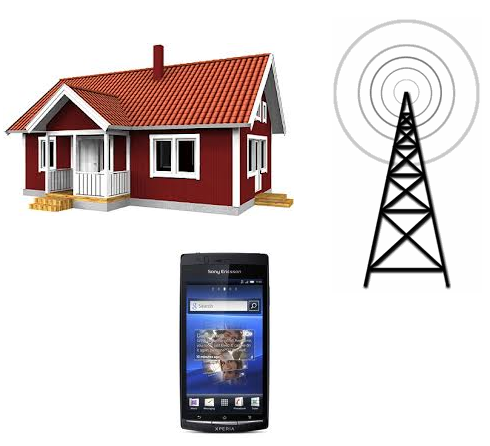
\includegraphics[width=\textwidth]{framsida.png}
\vfill
{\noindent {\Huge Sommarstugekoll} \\[0.1cm]
	\emph{\Large EDA234 - Digital ponstruktion, projektkurs} \\[1cm]
	
	{\large Grupp 1} \\ [.5cm]
	{\large Christian Isaksson}\\[.1cm]
	{\large Jan Pettersson}\\[.1cm]
	{\large Christoffer Öjeling}\\[2.4cm]
}

\end{titlepage}



%-----------------------------------------------------------

% Sammanfattning

\begin{abstract}
\begin{center}
\Large\sffamily{\textbf{Sammanfattning}}
\end{center}
\vspace{0.4cm}
Sommarstugekoll är en prototyp för avläsning av temperatur och reglering av element via SMS-kommunikation. Prototypen bygger på en FPGA, en extern temperatursensor och en mobiltelefon med serieinterface (RS232).
Genom att skicka fördefinierade kommandon finns möjligheten att slå av/på element eller begära temperaturen.
När ett sms tagits emot avkodas dess innehåll för att identifiera eventuella kommandon som getts till systemet och därefter utförs de.
Prototypen avslutar med att skicka en status rapport till avsändaren av sms:et.
\end{abstract}
\thispagestyle{empty}

%-----------------------------------------------------------

% Innehållsförteckning

\newpage
%\pagenumbering{roman}	% Romerska siffror som sidnumrering av innehållsförteckningen.
\setcounter{page}{1}

% Ta bort sidnummer från innehållsförteckningen.
\addtocontents{toc}{\protect\thispagestyle{empty}}

\tableofcontents


%-----------------------------------------------------------


\newpage
\pagenumbering{arabic}	



\section{Systemspecifikation} 
	Sommarstugekoll är ett system för övervakning och uppvärmning utav
	sommarstugor. Systemet  tillåter ägare att via sms få reda på inomhustemperatur och vilka
	element som är igång, samt möjligheten att slå av/på element i sommarstugan förutsatt att de
	är sammankopplade med detta system.
	\\\\
	När systemet får ett sms analyseras innehållet i sms:et för att identifiera eventuella kommandon
	till systemet. De kommandon som skickats till systemet kommer att utföras ett i taget, vilket
	innebär att om sms:ets avsändare både vill veta inomhustemperaturen och slå av/på element
	kommer först temperaturen att hämtas och därefter regleras elementen.  När alla kommandon
	utförts kommer huvudenheten att svara avsändaren med inomhustemperatur och alla elements
	nya status beroende på vilka kommandon avsändaren angett i sitt sms. Sen återgår systemet till
	vänteläget där det ligger och inväntar ett nytt sms.\\
	I det fall då sms:et saknar giltiga kommandon raderas det och huvudenheten går direkt tillbaka till
	vänteläget. 
	\\\\
	Systemet består huvudsakligen  utav tre delar, en huvudenhet,  en extern temperatursensor och en
	mobiltelefon med serieinterface (\emph{RS232}).  
	\\\\
	Huvudenheten är uppbyggd utav en \emph{Field-Programmable Gate Array} (FPGA) innehållande
	all logik.
\begin{figure}[H]
	\centering
	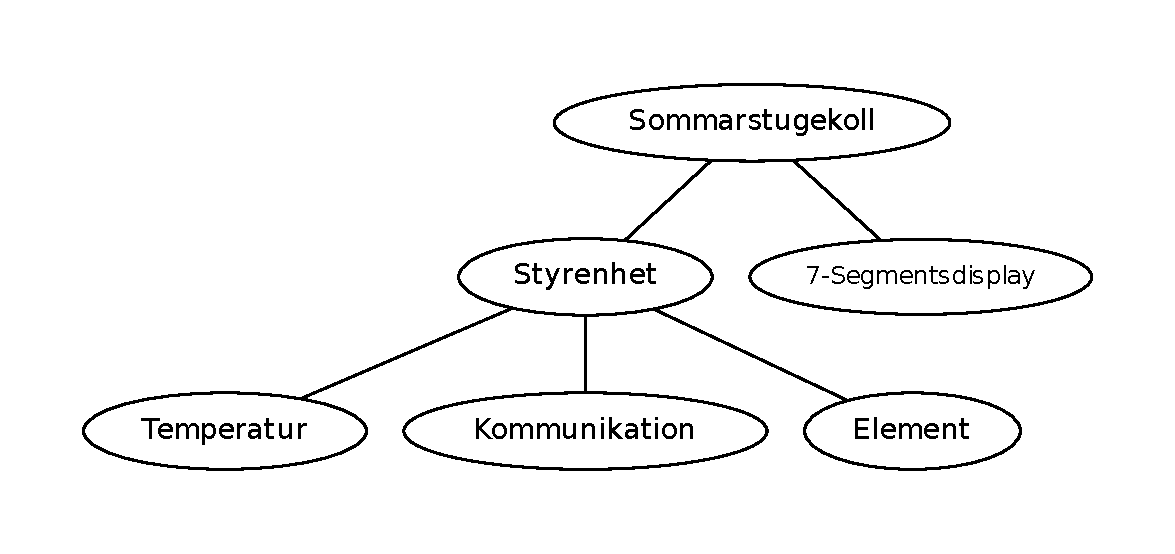
\includegraphics[width=\textwidth]{bigpicture.pdf}
	\caption{Övergripande struktur för projektet}
\end{figure}


\clearpage
\section{Systembeskrivning}

\subsection{Blockschema}
\begin{figure}[h!]
	\centering
	\advance\leftskip-3cm
	\advance\rightskip-3cm
	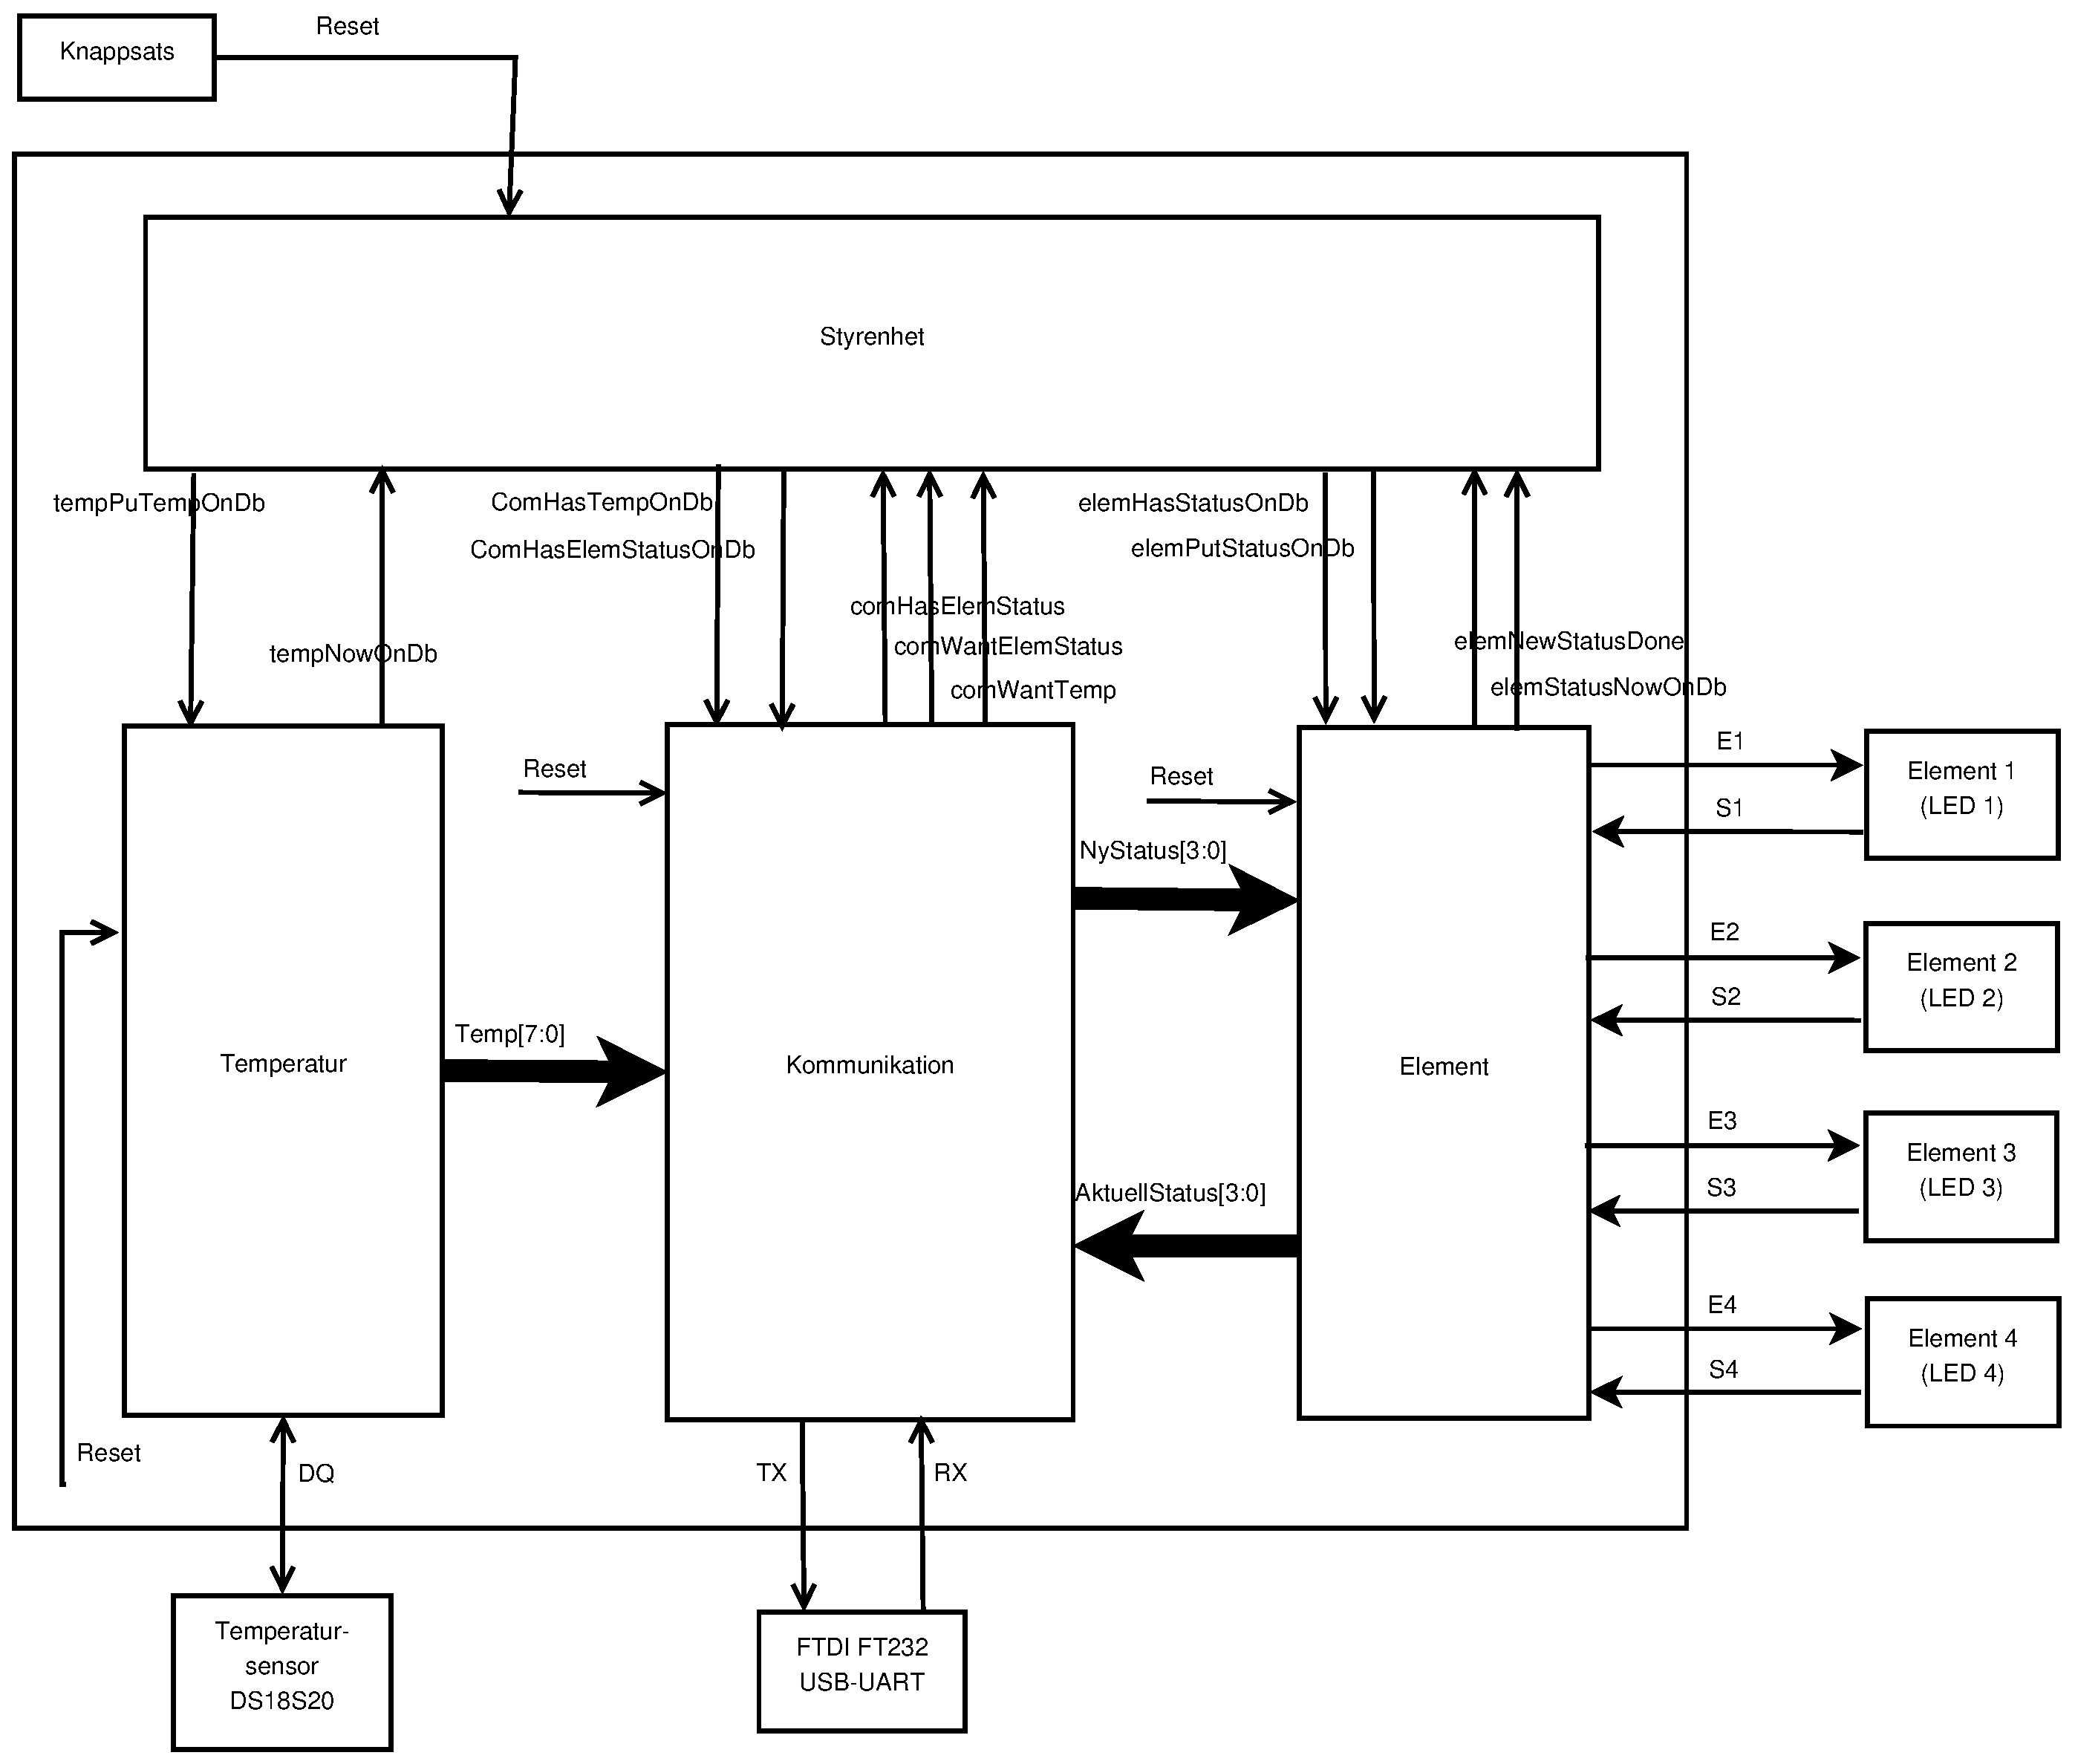
\includegraphics[width=15cm]{blockschema.eps}
	\caption{Övergripande blockschema för huvudenheten.}
\end{figure}


\clearpage
\section{Beskrivning av delblocken}

	\subsection{Styrenhet}
		Styrenheten tar emot insignaler från tre de delblocken: \emph{Element}, \emph{Kommunikation} och
		\emph{Temperatur}.
		\\
		Utifrån mottagna insignaler bestämmer styrenheten med hjälp av sina styrsignaler vilket delblock som ska läsa
		respektive skriva till databussen och om ett delblock förväntas skriva till databussen anger även styrsignalerna
		vad som ska skrivas. 
		\\\\
		Styrenheten bygger på en tillståndsmaskin med tre tillstånd: \textbf{Com}, \textbf{Temp} och \textbf{Elem}, där vardera
		av de tre tillstånd är kopplade till ett, och endast ett, utav de tre delblocken.
		
\begin{figure}[h!]
\centering
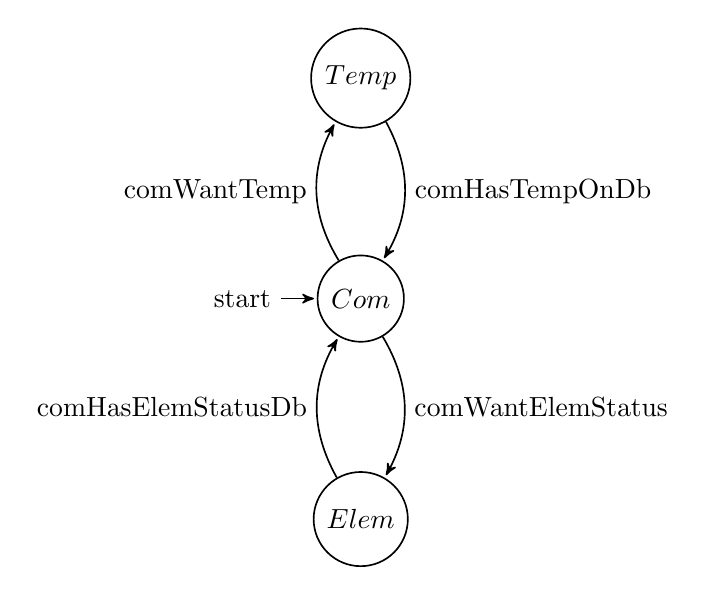
\begin{tikzpicture}[->,>=stealth',shorten >=1pt,auto,node distance=2.8cm,semithick]

\node[initial,state]	(A)				 {$Com$};
\node[state]		(B) [above of = A]		{$Temp$};
\node[state]		(C) [below of = A]		{$Elem$};

\path
	(A)	edge [bend left]	node {comWantTemp} (B)
		edge [bend left]	node {comWantElemStatus} (C)
	(B)	edge [bend left]	node {comHasTempOnDb} (A)
	(C)	edge [bend left]	node {comHasElemStatusDb} (A);
\end{tikzpicture}

\caption{Händelseförlopp för styrenheten.\\Namnen på bågarna mellan olika tillstånd anger signaler som ettställs vid tillståndsförändringen.}
\end{figure}

		
		I \textbf{Com} ligger styrenheten och väntar på kommandon från delblocket \emph{Kommunikation}.
		\\
		Om en begäran att få veta inomhustemperaturen fås, kommer styrenheten att byta tillstånd till \textbf{Temp} och med hjälp av
		en styrsignal meddela delblocket \emph{Temperatur} om att temperaturen ska inhämtas och skrivas till databussen.
		\\
		I det fall en begäran fås om att ändra elementens status, dvs. slå av/på ett eller flera element, skriver delblocket \emph{Kommunikation}
		den nya elementstatusen till databussen och sedan meddelas styrenheten om att ny status finns att läsa på databussen. Därefter
		ändras tillstånd till \textbf{Elem}.
		\\
		Om enbart information om elements aktuella status begärs, sätts styrenhetens styrsignaler till att meddela \emph{Element}
		att enbart aktuella element status behöver skrivas till databussen samtidigt som en tillståndsövergång till \textbf{Elem} sker.
		\\\\
		I \textbf{Temp} väntar styenheten på kvittens från \emph{Temperatur} om att temperaturen skrivits till databussen
		och går att läsa.
		\\
		När kvittens fåtts återgår styrenheten till tillståndet \textbf{Com}, samtidigt som en styrsignal meddelar delblocket \emph{Kommunikation}
		att temperaturen nu finns att hämta på databussen.
		\\\\
		I \textbf{Elem} väntar styrenheten på kvittens från delblocket \emph{Element} om att elementen har reglerats och/eller
		att aktuell elementstatus finns på databussen.
		\\
		När kvittens fåtts återgår styrenheten till tillståndet \textbf{Com}, samtidigt som styrsignaler meddelar delblocket \emph{Kommunikation}
		att elementen reglerats och/eller aktuell elementstatus finns att hämta på databussen.
		
	
\subsection{Temperatur}\label{sec:temperatur}
Logiken för avläsning av temperatur är uppdelad i ett antal delblock. Dels för att vara lättöverskådligt, men även så att man lätt ska kunna lägga till funktionalitet i efterhand. Slutanvändaren använder endast \nameref{sec:ds18s20} direkt. Onewire modulen är inte bunden till just DS12S20, utan kan även användas till andra andra enheter som använder sig utav 1-wire protokollet.

All logik använder sig utav VHDL-standardbiblioteket \signal{numeric\_std} för hantering av tal med och utan tecken.

%%% DS18S20 %%%%%%%%%%%%%%%%%%%%%%%%%%%%%%%%%%%%%%%%%%%%%%%%%%%%%%%%%
\subsubsection{DS18S20}\label{sec:ds18s20}
\paragraph{Interface}
DS18S20 exponerar ett interface för mätning och avläsning av nuvarande temperatur. Mätningen initieras genom att \signal{measure} sätts till \signal{'1'}. När temperaturmätningen är klar kommer \signal{valid} sättas till \signal{'1'}.
Då finns temperaturen att avläsa på \signal{temperature} som ett binärt 8 bitars tal på tvåkomplementsform där där bit 7--1 är heltalsdelen och bit 0 decimaldelen.
\signal{valid} fortsätter att vara \signal{'1'} tills en ny mätning initieras genom att \signal{measure} återigen sätts till \signal{'1'}.

En temperaturmätning tar upp till 750ms.
\begin{figure}[htp]
\centering
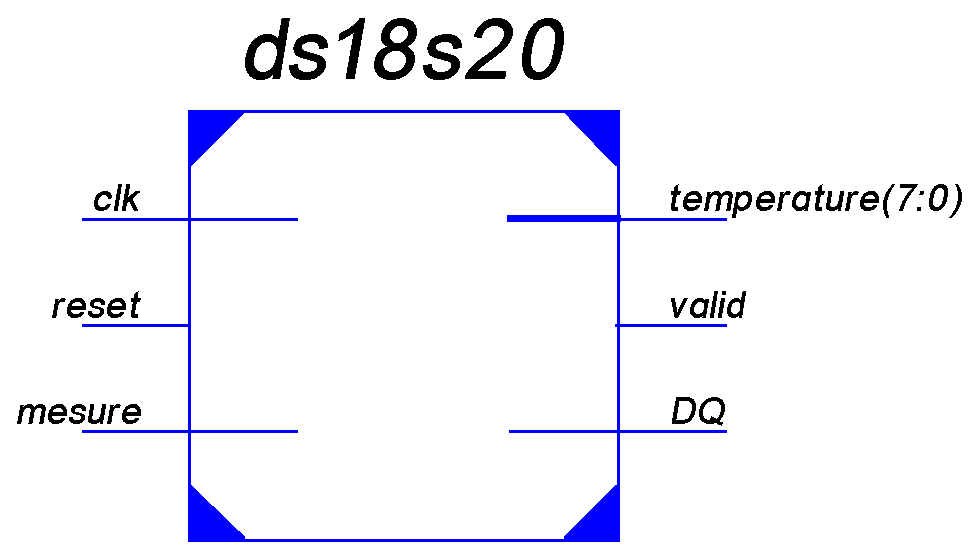
\includegraphics[scale=0.5]{ds18s20_sch.eps}
\caption{Delblocket DS18S20}
\end{figure}

\paragraph{Implementation}
Själva logiken i sig består av en cirkulär tillståndsmaskin (\autoref{fig:ds18s20_fsm}).
Tillståndsmaskinen växlar mellan att ge olika kommandon till onewire-blocket, och sedan vänta på att kommandot ska utföras. En mer utförlig beskrivning när data avläses och hur det samplas finns under \ref{sec:onewire} \nameref{sec:onewire}.
DS18S20 har stöd för flera sensorer på samma buss. De delar då DQ och varje sensor har unikt serienummer för identifiering. I denna konstruktion används endast en sensor och logik för identifiering av flera sensorer utelämnas.

VHDL koden är uppbyggd efter tvåprocessmodellen, med en klockad och en kombinatorisk process.


\begin{table}[H]

\begin{tabularx}{\textwidth}[h]{c c X}
	\hline
	\textbf{Master} & \textbf{Data} & \textbf{Kommentar} \\
	\hline
	
	\Tx & Reset & Reset puls.\\
	\Rx & Presence & Sensorn svarar med en presence puls.\\
	\Tx & 0x44 & Skip ROM command. Eftersom det bara finns en sensor på bussen skippas identifiering.\\
	\Tx & 0x44 & Convert T command. Sensorn mäter och sparar nuvarande temperatur till sitt interna minne.\\
	\Rx & & Sensorn pollas kontinuerligt tills den svarar \high{}, vilket indikerar att mätningen är klar.\\
	\Tx & Reset & Reset puls.\\
	\Rx & Presence & Sensorn svarar med en presence puls.\\
	\Tx & 0x44 & Skip ROM command. Eftersom det bara finns en sensor på bussen skippas identifiering.\\
	\Tx & 0xBE & Read scratchpad command. Läser sensorns interna minne.  \\
	\Rx & <1 byte> & Läser första byten vilket är temperaturen.\\
	
	\hline
\end{tabularx}
\caption{Kontrollsekvens för mätning och avläsning av temperatur}
\end{table}


\begin{figure}[h!]
	\centering
	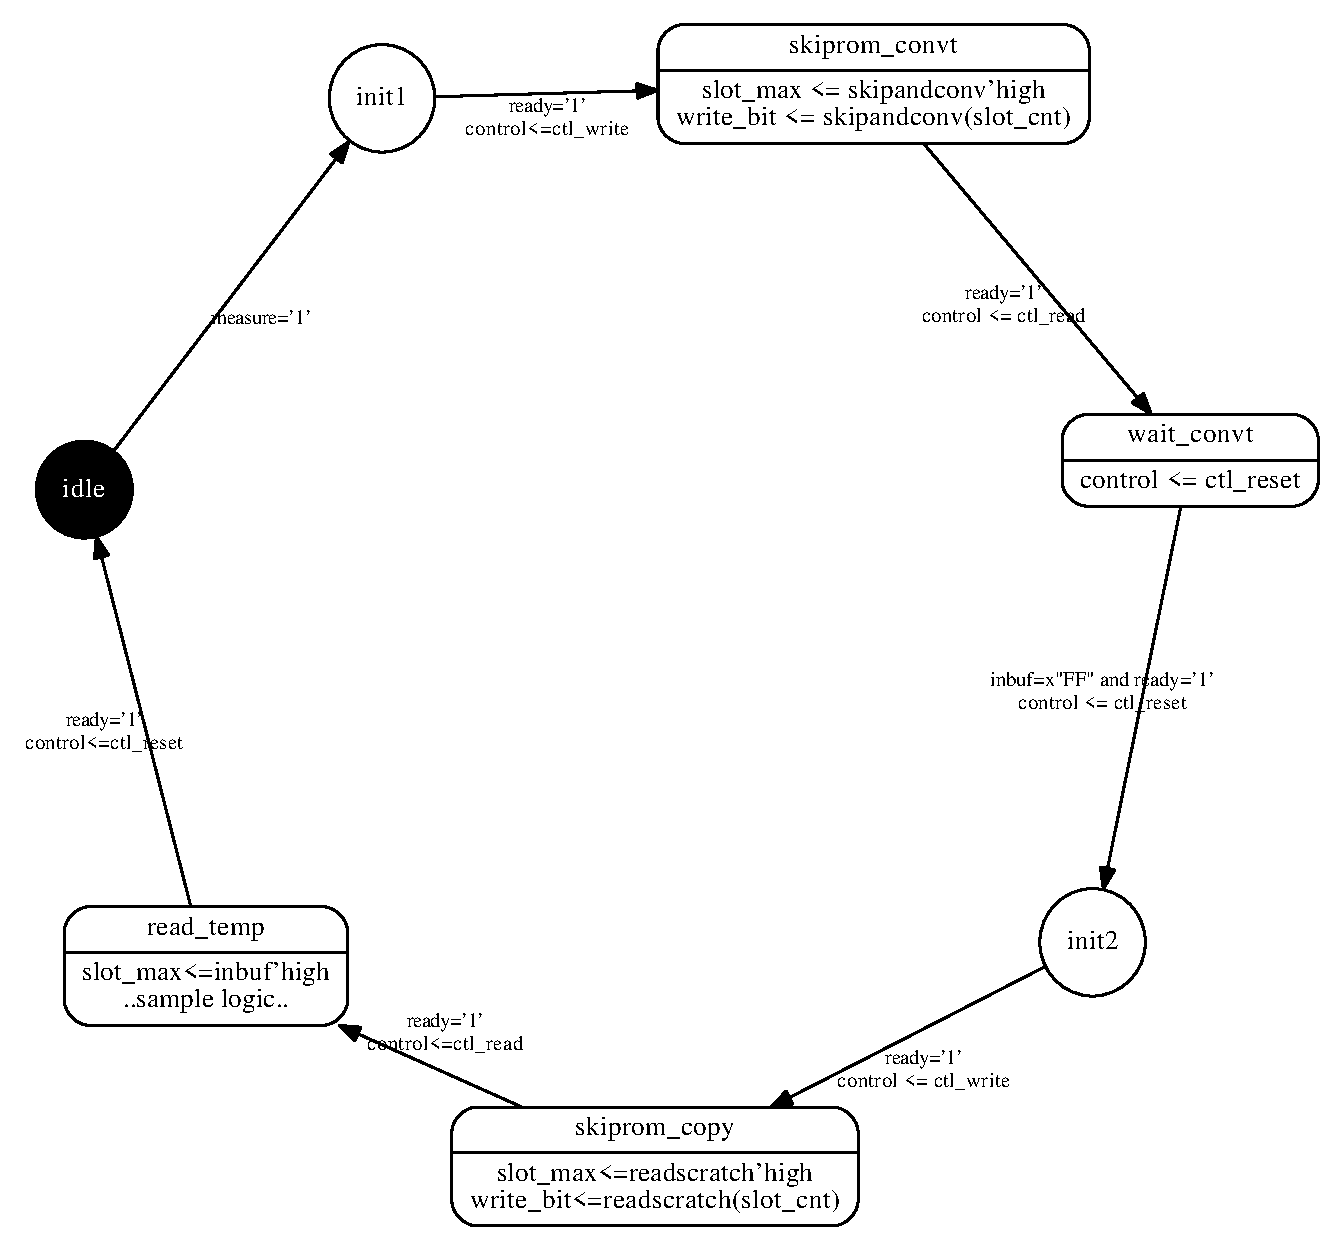
\includegraphics[width=\textwidth]{ds18s20_fsm.eps}
	\caption{Tillståndsmaskin för delblocket DS18S20}
	\label{fig:ds18s20_fsm}
\end{figure}



\subsubsection{Onewire}\label{sec:onewire}
\paragraph{Interface}
Delblocket onwire sköter lågnivå kommunikationen med temperatursensorn, och exponerar ett högre nivå interface med fyra kontroll-kommandon och en ready signal. För att initiera en operation sätts \signal{control} signalen till ett av följande värden när \signal{ready='1'}:

\begin{description}
\item[ctl\_idle] Gör ingenting. \signal{ready} kommer konstant vara \signal{'1'}.

\item[ctl\_read] Läs \signal{slot\_max} antal bitar från sensorn. \signal{slot\_cnt} är en räknare som indikerar vilken bit som läses just nu. När \signal{sample\_now='1'} Förväntas användaren spara biten som under den klockcykeln finns på \signal{read\_bit}. När alla bitar är lästa kommer \signal{ready} sättas till \signal{'1'}.

\textbf{Exempel:}
\begin{lstlisting}
if rising_edge(clk) then
	if sample_now = '1' then
		in_buffer(slot_cnt) <= read_bit;
	end if;
end if;
\end{lstlisting}


\item[ctl\_write] Skriv \signal{slot\_max} antal bitar till sensorn. \signal{slot\_cnt} är en räknare som indikerar vilken bit som skrivs just nu. Användaren förväntas lägga biten som ska skrivas till sensorn på \signal{write\_bit}.
När alla bitar är skrivna kommer \signal{ready} sättas till \signal{'1'}.

\textbf{Exempel:}
\begin{lstlisting}
write_bit <= out_buffer(slot_cnt);
\end{lstlisting}

\item[ctl\_reset] Återställer sensorns tillståndsmaskin.
När reset-sekvensen är klar kommer \signal{ready} sättas till \signal{'1'}.


\end{description}
Under en pågående operation kommer \signal{ready} vara \signal{'0'}.
Observera att efter ``power on'' eller ``master reset'' kommer onewire utföra reset-sekvensen för sensorn, och användaren måste vänta på \signal{ready='1'} innan ett kontrollkommando kan ges.
Det finns även en \signal{error} signal som kommer gå hög under en klockcykel om inte temperatursensorn svarar under resetsekvensen.
\begin{figure}[H]
	\centering
	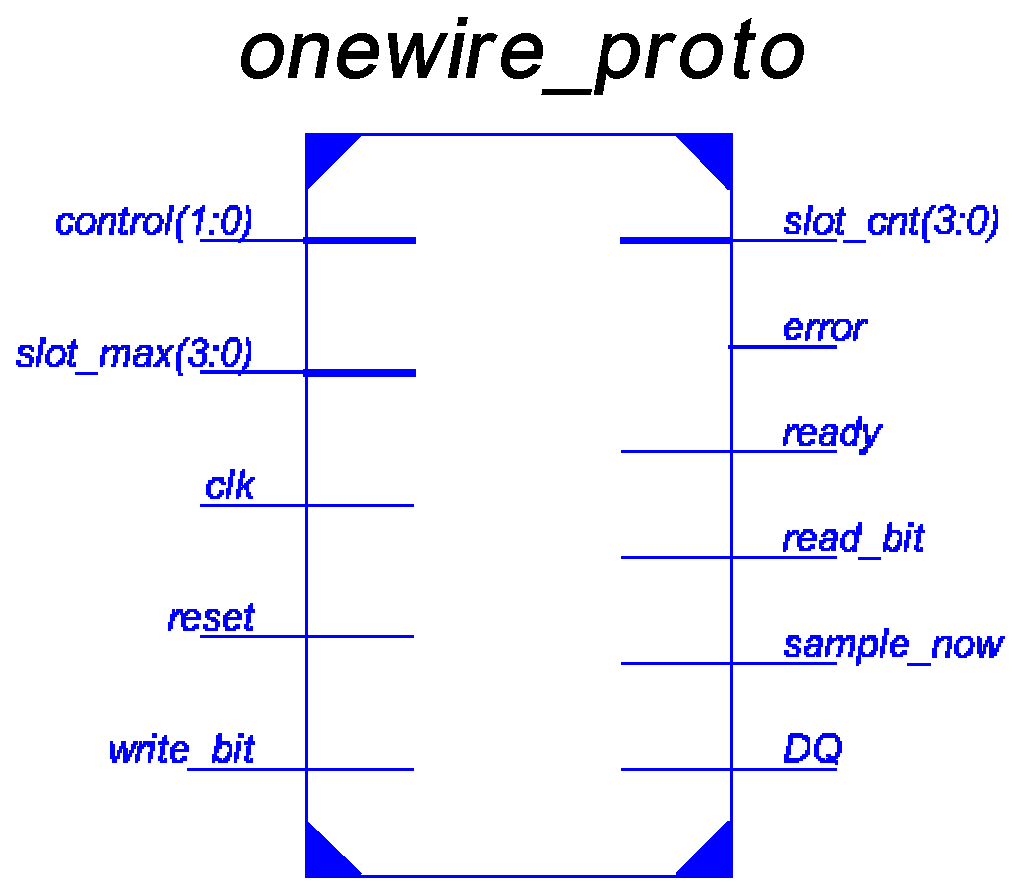
\includegraphics[scale=0.5]{onewire_sch.eps}
	\caption{Delblocket onewire}
\end{figure}

\paragraph{Implementation}
Onewire delblocket implementerar Dallas 1-wire protokoll. För 1-wire används enbart en pin (DQ) för kommunikation. Ingen gemensam klocka finns. 1-wire bygger på master-slave principen, med sensorn som slave och kontrollen som master. Till DQ är en 5K\ohm pullup resistor kopplad. Kommunikation sker via \emph{write slots} och \emph{read slots}. Mastern initierar all kommunikation. 1-wire är \emph{open drain}, vilket innebär att pullup resistorn driver DQ hög när det inte är någon aktivitet på bussen. All data skrivs och avläses med den minst signifikanta biten först (LSB).

1-wire har stöd för sk. ``parasite power'', där DQ driver temperatursensorn. Onewire delblocket använder sig dock inte utav denna funktion, utan sensorn drivs genom $V_{dd}$.

Kontrollen är uppbyggd av en tillståndsmaskin, se \autoref{fig:onewire_fsm}. VHDL koden är uppbyggd efter tvåprocessmodellen, med en klockad och en kombinatorisk process.

\begin{figure}[H]
\centering
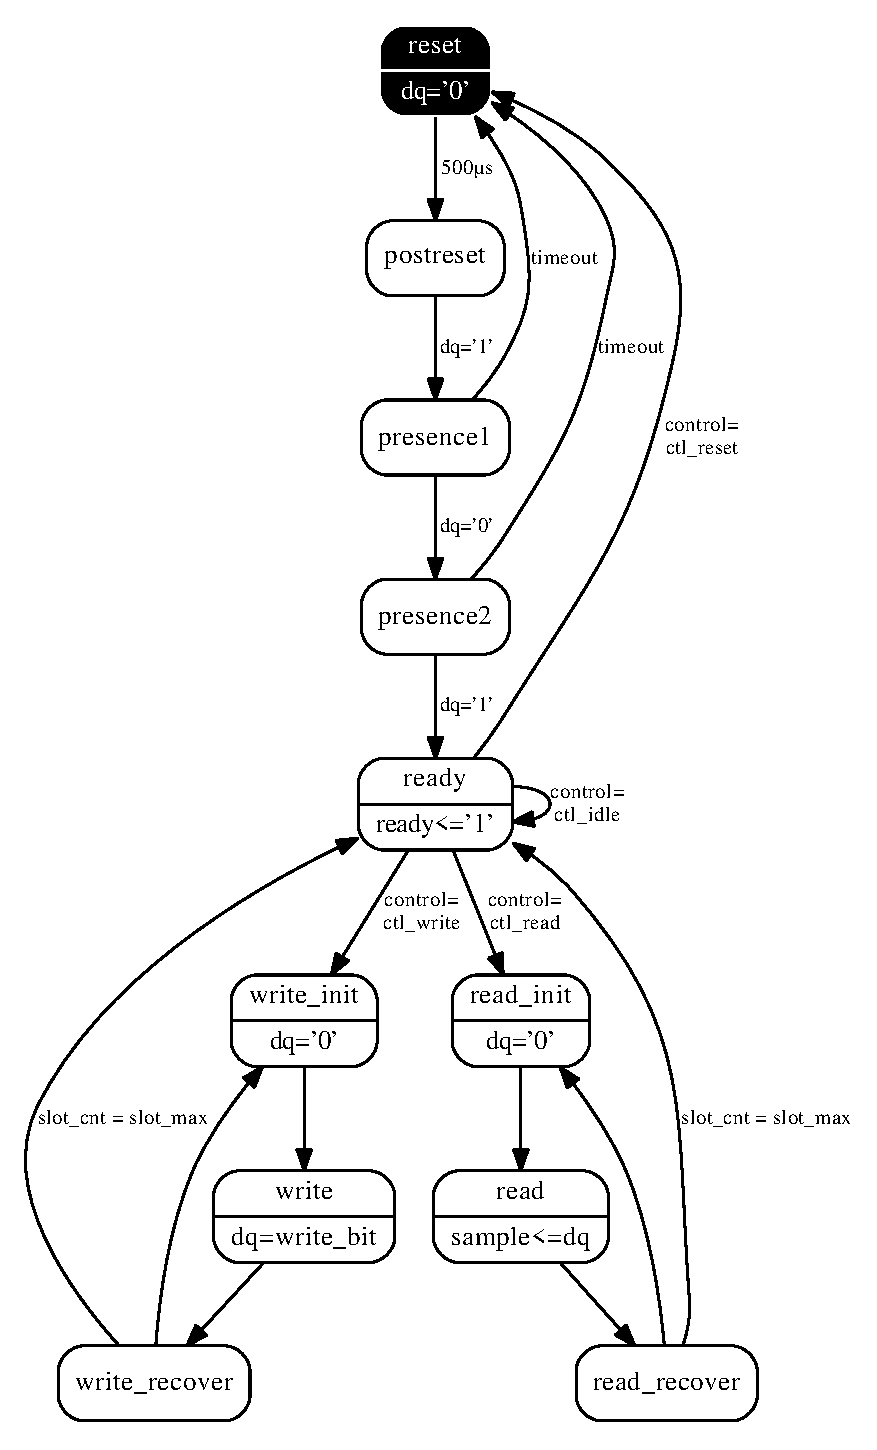
\includegraphics[height=0.97\textheight]{onewire_fsm.eps}
\caption{Tillståndsmaskin för delblocket onewire}
\label{fig:onewire_fsm}
\end{figure}


\subparagraph{Reset}
Resetfasen korresponderar till $reset\rightarrow postreset\rightarrow presence1\rightarrow presence2\rightarrow ready$ i onewires tillståndsmaskin (\autoref{fig:onewire_fsm}).

Vid FPGAns \emph{power on}, eller när den globala, asynkrona \signal{reset} signalen går från hög till låg kommer tillståndsmaskinen börja i \state{reset}. Initieringssekvensen för temperatursensorn DS18S20 kommer då inledas. Se \autoref{fig:ow_timings}. Om temperatursensorn svarar med en korrekt \emph{presence pulse} inom accepterade tidsintervall kommer onewire att försättas i tillstånd \state{ready} och invänta vidare kommandon. Vid felaktikt eller uteblivet svar kommer \signal{error} vara \high{} under en klockcykel. Tillståndsmaskinen kommer sedan återgå till \state{reset} och börja om initieringssekvensen.

\begin{figure}[H]
	\centering
	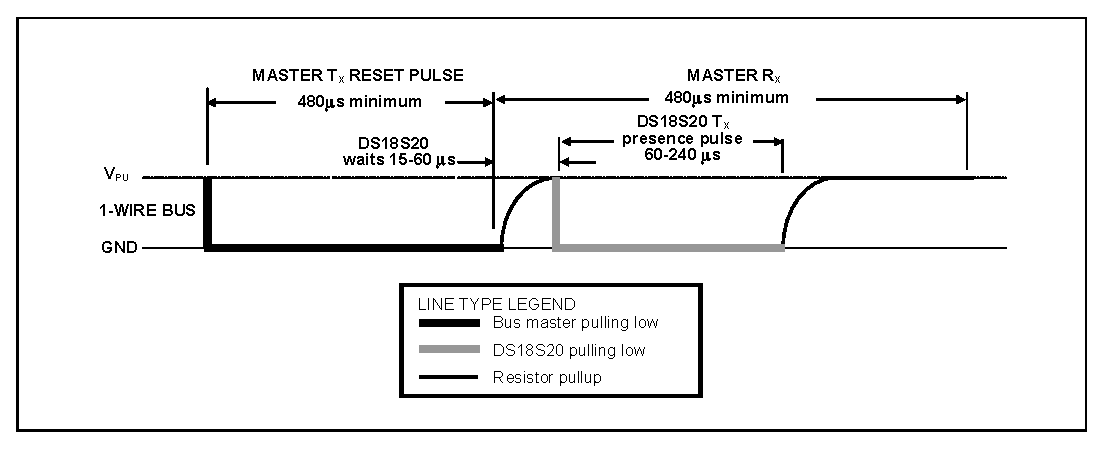
\includegraphics[width=\textwidth]{reset_presence.eps}
	\caption{Timings för 1-wire resetsekvens}
	\label{fig:ow_timings}
\end{figure}


\subparagraph{Skrivning med \emph{write slots}}
Skrivfasen korresponderar till $ready\rightarrow write\_init\rightarrow write\rightarrow write\_recover$ i onewires tillståndsmaskin (\autoref{fig:onewire_fsm}).

För att påbörja en skrivning sätts \signal{control} till \signal{ctl\_write} när \signal{ready='1'}.
\signal{slot\_max} bitar kommer då skrivas till sensorn.
1-wire protokollet anvander \emph{write slots} för att skriva bitar till sensorn. Flera bitar skrivs genom flera efterföljande write slots.

En write slot börjar med att buss-mastern driver DQ låg 1--15\us. Sensorn kommer sampla värdet på bussen 15--60\us efter att DQ gick från hög till låg. Efter varje write slot behövs >1\us återhämtningstid.

För att skriva \low{} driver kontrollen DQ låg i 60\us{} < \Tx{} < 120\us{}.
För att skriva \high{} släpper kontrollen DQ maximalt 15\us{} efter att write slot påbörjades.
Se \autoref{fig:rwslots}.


\subparagraph{Läsning med \emph{read slots}}
Läsfasen korresponderar till $ready\rightarrow read\_init\rightarrow read\rightarrow read\_recover$ i onewires tillståndsmaskin (\autoref{fig:onewire_fsm}).

För att påbörja en läsning sätts \signal{control} till \signal{ctl\_read} när \signal{ready='1'}.
\signal{slot\_max} bitar kommer då läsas från sensorn.
1-wire protokollet anvander \emph{read slots} för att skriva bitar till sensorn. Flera bitar skrivs genom flera efterföljande read slots.
En read slot intitieras alltid av mastern genom att driva DQ låg i 1\us{} < \Tx{} < 15\us{}. Sensorn kommer efter att DQ gått från \high{} $\rightarrow$ \low{} lägga ut \high{} eller \low{} på DQ. Data är giltig upp till 15\us{} efter det att master initierar read slot.
Se \autoref{fig:rwslots}.



\begin{figure}
\centering
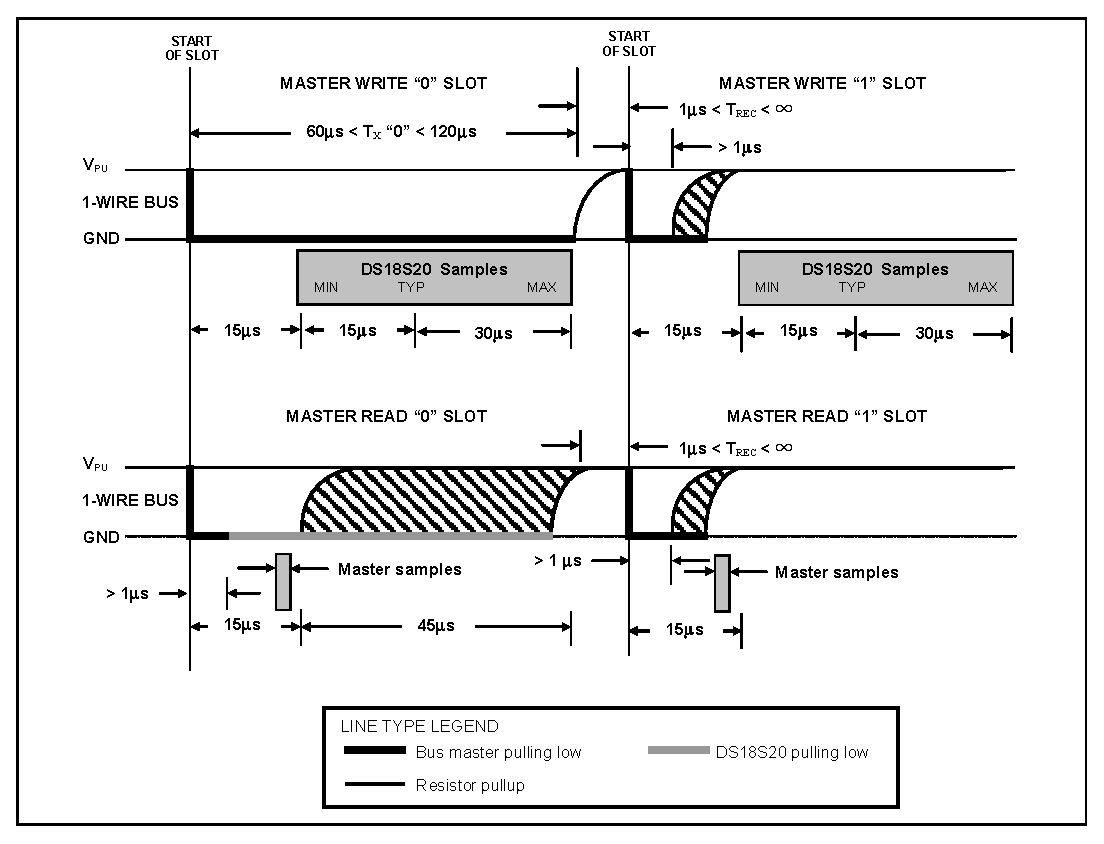
\includegraphics[width=\textwidth]{write_slot.eps}
\caption{Write och read slots timings för \low{} respektive \high{}.}
\label{fig:rwslots}
\end{figure}



%%% 7-segmentsdisplay %%%%%%%%%%%%%%%%%%%%%%%%%%%%%%%%%%%%%%%%%%%%%%%%%%%%%%%%%%%
\subsection{7-Segmentsdisplay}\label{sec:7seg}
Delblocket ansvarar för att visa ett 8 bitars binärt tal på tvåkomplementsform där bit 7--1 är heltalsdelen och bit 0 decimaldelen på en 7-segmentsdisplay med basen 10.

Det finns stöd för att visa tal mellan -99 -- 999, med en decimalsiffra som antingen är .0 eller .5. Det är tillräckligt för temperatursensorn som är specifierad mellan $-75 -- 125 \pm5$.
\subsubsection{segment\_temperature}

\paragraph{Interface}
Komponenten tar ett binärt tal som input och ger utsignalerna till 7-segmentsdisplayerna.

<bild>

\paragraph{Implementation}
De fyra fysiska 7-segmentsdisplayerna har en gemensam databuss. Varje display har även en enable signal. Komponenten växlar mellan att visa de olika displayerna med 1kHz, vilket för ögat upplevs som att alla lyser konstant.
\paragraph{bcd}\label{sec:bcd}
Funktion som gör om ett binärt tal utan tecken till bcd-form. ``Double Dabble'' algoritmen används internt i form utav ett kombinatoriskt nät.


\begin{figure}[htp]
\centering
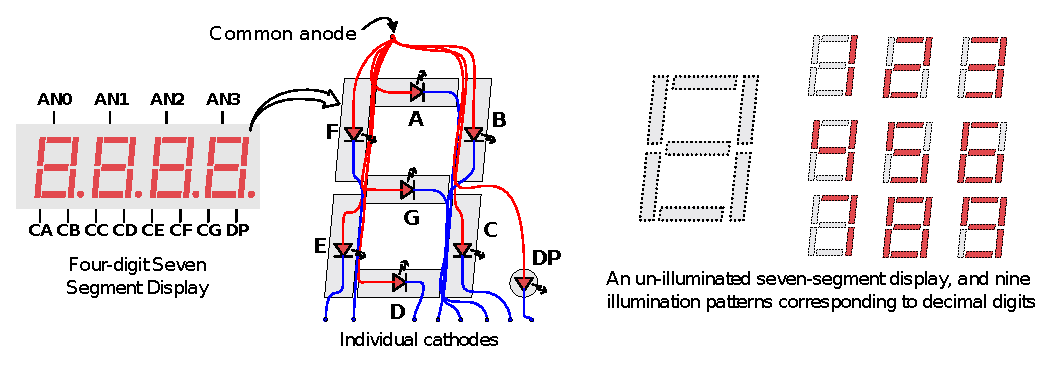
\includegraphics[width=\textwidth]{segment.eps}
\caption{7-segments display}
\label{}
\end{figure}
	\subsection{Kommunikation}

	\subsection{Element}
		Detta block hanterar allt som har med elementen att göra.
		\\
		Blocket sparar även sitt tillstånd, vilket innebär att det själv är medvetet om vilka element som är av- och påslagna.
		\\\\
		Först kontrolleras insignalerna för att avgöra om ett eller flera elemenet ska regleras och/eller om elementens aktuella status ska
		skrivas till databussen.
		\\
		Om elementen ska regleras hämtas ny status från databussen och sedan slås elementen av/på beroende på vad som står i datan som hämtats
		från databussen.
		\\
		Önskas aktuell elementstatus, eller ny elementstatus i det fall att elementen har reglerats, skrivs den till databussen.
		\\
		Efter att elementen har reglerats och/eller aktuell elementstatus skrivits till databussen sätts utsignaler för att tala om exakt
		vad som gjorts.

		
		
\clearpage
\section{Hårdvara}\label{sec:hårdvara}
	Systemet är uppbyggt utav huvudsakligen tre komponenter: ett Digilent Nexys3 utvecklingskort, en
	temperperatursensor från Maxim och en mobiltelefon med serieinterface (\emph{RS232}).

	\subsection{Digilent Nexys3 - FPGA}
		Nexys3 är ett utvecklingkort från Digilent som bygger på en Spartan-6 FPGA från Xilinx.
		\\
		\textbf{Nexys3 har bland annat:}
		\begin{itemize}
			\item Xilinx Spartan-6 XC6SLX16 CSG324C.
			\item Klockfrekvens på 100MHz.
			\item 48MB externt minne, varav 32MB är ickeflyktigt.
			\item Mikro USB-port för programmering av FPGA och strömförsörjning.
			\item USB-UART, genom en mikro USB-port kopplad vid en FTDI FT232 krets.
			\item USB Host-kontroller för anslutning utav externa USB-enheter, ex. mus, tangentbort, osv.
			\item 10-100 Mbit ethernet-anslutning.
			\item 4st sjusegments displayer.
			\item 8st binära DIP switchar.
			\item 8st ytmonterade lysdioder
			\item 4st kontaktstycken för externa I/O-enheter (dubbelbreda Pmod anslutningar).
		\end{itemize}
		
		
		
		

\subsection{DS18S20 - Temperatursensor}
DS18S20 är en temperatursensor tillvärkad av Dallas Semiconductor (numera Maxim) som enbart använder sig utav 1 pin för kommunikation. 
\\
\textbf{Sensorn har:}
\begin{itemize}
	\item Temperaturmätning från -75\degcel{} till 125\degcel{} med $\pm5$ precision.
	\item Alarmfunktion med icka-flyktigt minne.
	\item Max 750ms för temperaturmätning
	\item Flera sensorer kan dela på en buss.
	\item Ett unikt för varje enhet 64 bitars serienummer.
	\item Endast två pinnar behövs om ``parasite power'' anvands. Då laddar sensorn upp en kondensator när DQ drivs aktivt hög.
\end{itemize}
\begin{figure}[htp]
	\centering
	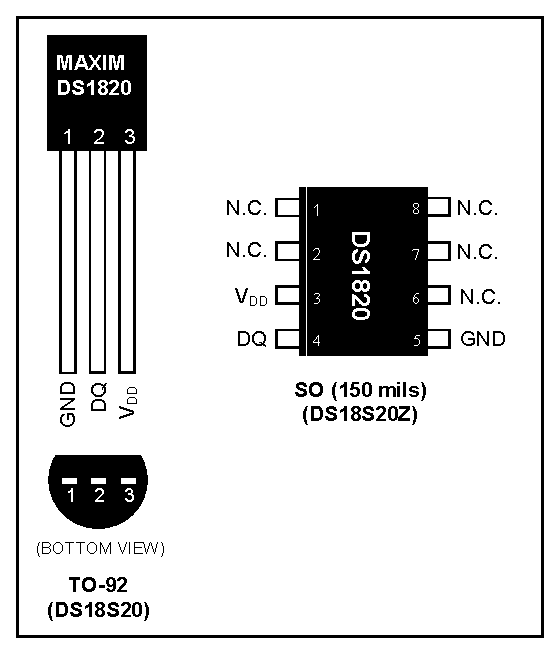
\includegraphics[scale=0.8]{ds18s20_hardware.eps}
	\caption{Dallas DS18S20}
\end{figure}



	
\clearpage
\section{Resultat och diskussion}

\subsection{Resultat}

\subsection{Felanalys}

\subsection{Diskussion}


\clearpage
\appendix
\pagenumbering{roman}

\clearpage
\section{Kommandon}
\begin{table}[H]
		\begin{tabularx}{\textwidth}{l X}
			\hline
			\textbf{Kodord}     & \textbf{Funktion} \\
			\hline
			get element	&	Begär antal element som är igång.\\
			get temp	&	Begär nuvarande temperatur\\
			set element:<element[int]		& Sätter antal element som ska vara igång\\
			\hline
			temp:<temp[int]>	& Anger nuvarande temperatur\\
			element:<element[int]> &	Anger antal element igång\\
		\end{tabularx}
\end{table}

\begin{table}[H]
		\begin{tabularx}{\textwidth}{p{2cm} X p{5cm}}
			\hline
			\textbf{Avsändare}  & \textbf{AT-kommando}     & \textbf{Funktion}\\
			\hline
			GSM-enhet	&	+CMTI=<mem. location>,<index>						&	Anger index för nytt meddelande. \\
			AT-modul	&	AT+CMGF=1										&	Ställer in 'text mode' på GSM modulen.\\
			AT-modul	&	AT+CMGR=<index>								&	Begär meddelandet med angivet index.\\
			GSM-enhet	&	+CMGR:``REC READ'',``<telefon nr.>''``<datum>'' <kodord> <OK>	&  	Meddelandet med data och kodord från användaren.\\
			AT-modul	&	AT+CMGS="<telefon nummer>" <data> 					&	Meddelande innehållandes svarsdata till användaren.\\
		\end{tabularx}
\end{table}

\section{Signallista}
\subsection{DS18S20}
\begin{table}[H]
	\begin{tabularx}{\textwidth}{p{2cm} p{4.3cm} X}
		\hline
		\textbf{Namn} & \textbf{Typ} & \textbf{Kommentar} \\
		\hline
		clk & in std\_ulogic & Global klocka, 100MHz \\
		reset & in std\_ulogic & Global asynkron reset \\
		measure & in std\_ulogic & Påbörja temperaturavläsning \\
		valid & buffer std\_ulogic & Temperaturavläsning klar. 
			Giltig så länge \signal{valid = '1'} \\
		DQ & inout std\_logic & Pinne till sensor \\
		temperature & buffer signed(7 downto 0) & Temperatur i tvåkompliments binärform \\
		\hline
	\end{tabularx}
\end{table}


\subsection{segment\_temperature}
\begin{table}[H]
	\begin{tabularx}{\textwidth}{p{2cm} p{4.3cm} X}
		\hline
		\textbf{Namn} & \textbf{Typ} & \textbf{Kommentar} \\
		\hline
		clk & in std\_ulogic & Global klocka, 100MHz \\
		reset & in std\_ulogic & Global asynkron reset \\
		rawd & in signed(7 downto 0) & Temperatur i tvåkompliments binärform \\
		valid & out std\_ulogic & Temperaturavläsning klar. 
			Giltig så länge \signal{valid = '1'} \\
		an & buffer std\_ulogic\_vector(3 downto 0) & 7 Segment-enable \\
		segment & buffer std\_ulogic\_vector(7 downto 0) & Utsignal till 7 segmentsbussen \\
		\hline
	\end{tabularx}
\end{table}

\subsection{Com}
\begin{table}[H]
	\begin{tabularx}{\textwidth}{p{2cm} p{4.3cm} X}
		\hline
		\textbf{Namn} & \textbf{Typ} & \textbf{Kommentar} \\
		\hline
		clk & in std\_ulogic & Global klocka, 100MHz \\
		rst & in std\_ulogic & Global asynkron reset \\
		tempInAvail & in std\_logic & Temperatur finns tillgänlig på bus\\
		elementInAvail & in std\_logic & Elementdata finns tillgänlig på bus\\
		requestTemp & out std\_logic & Ber styrenheten om tempdata till bus\\
		requestElement & out std\_logic & Ber styrenheten om elementdata till bus\\
		elementOutAvail & out std\_logic & Meddelar styrenheten, elementdata på bus\\
		tempIn & in std\_logic\_vector(7 downTo 0) & Databus från temperaturmodul\\
		elementIn & in std\_logic\_vector(1 downTo 0) & Databus från elementmodul \\
		elementOut & out std\_logic\_vector(7 downTo 0) & Databus till elementmodul\\
		tx & out std\_logic & Seriel port ut till GSM enhet ut från AT-modul\\
		rx & in std\_logic & Seriel port in till AT-modul från GSM-modul\\		
		\hline
	\end{tabularx}
\end{table}



\clearpage
\section{Kretsschema}
	\begin{figure}[H]
	\centering
	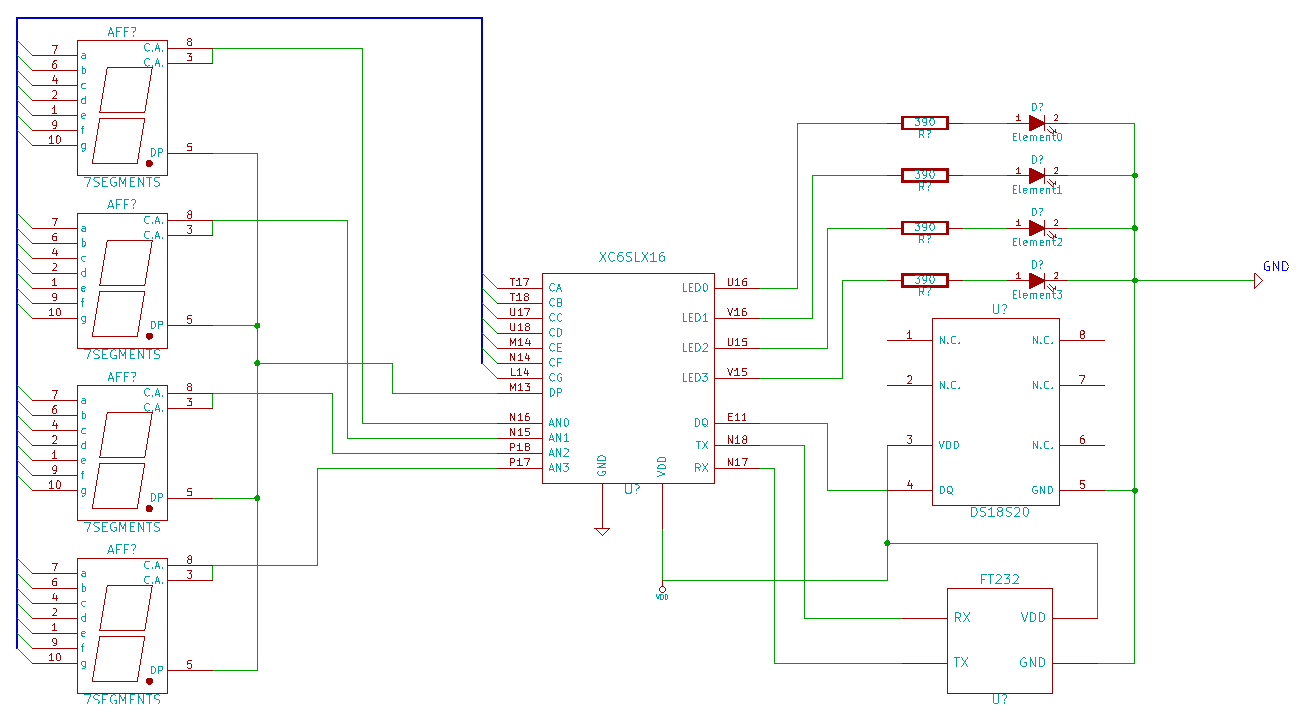
\includegraphics[width=0.88\textheight, angle=90]{kretsschema.eps}
	\caption{Förenklat kretsschema, över de komponenter som används, baserat på Digilents kretsschema för Nexys3.}
	\label{}
\end{figure}


\clearpage
\section{Syntesschema}

\clearpage
\section{Komponentlista}
\begin{table}[H]
		\begin{tabularx}{\textwidth}{l X}
			\hline
			\textbf{Namn}     & \textbf{Beteckning} \\
			\hline
			Utvecklingskort	&	Digilent Nexys3	\\
			Temperatursensor	&	Maxim DS18S20	\\
			Motstånd			&	4.7 k\ohm{}	\\
			\hline
		\end{tabularx}
\end{table}

\newpage

\section{Pinlayout}
	\begin{table}[H]
		\begin{tabularx}{\textwidth}{l X l l}
			\hline
			\textbf{Pin} & \textbf{Beskrivning} & \textbf{Från} & \textbf{Till}\\
			\hline
			T17 & Katod för segment A & FPGA & 7-segmentsdisplayen\\
			T18 & Katod för segment B & FPGA & 7-segmentsdisplayen\\
			U17 & Katod för segment C & FPGA & 7-segmentsdisplayen\\
			U18 & Katod för segment D & FPGA & 7-segmentsdisplayen\\
			M14 & Katod för segment E & FPGA & 7-segmentsdisplayen\\
			N14 & Katod för segment F & FPGA & 7-segmentsdisplayen\\
			L14 & Katod för segment G & FPGA & 7-segmentsdisplayen\\
			M13 & Katod för segment DP & FPGA & 7-segmentsdisplayen\\
			N16 & Gemensam anod för 7-seg AN0 & FPGA & 7-segmentsdisplayen\\
			N15 & Gemensam anod för 7-seg AN1 & FPGA & 7-segmentsdisplayen\\
			P18 & Gemensam anod för 7-seg AN2 & FPGA & 7-segmentsdisplayen\\
			P17 & Gemensam anod för 7-seg AN3 & FPGA & 7-segmentsdisplayen\\
			U16 & Aktivera lysdiod LD0 & FPGA & LED0\\
			V16 & Aktivera lysdiod LD1 & FPGA & LED1\\
			U15 & Aktivera lysdiod LD2 & FPGA & LED2\\
			V15 & Aktivera lysdiod LD3 & FPGA & LED3\\
			N18 & Tx & FPGA & USB-UART FTDI FT232\\
			N17 & Rx & FPGA & USB-UART FTDI FT232\\
			\hline
		\end{tabularx}
	\end{table}


\clearpage
\section{Programkod (VHDL)}
All programkoden inklusive testfiler finns i ett git-källkodsrepository:
\begin{lstlisting}[	language=VHDL, basicstyle=\ttfamily]
https://github.com/Cadynum/sommarstuga.git
\end{lstlisting}

\begin{figure}[htp]
\centering
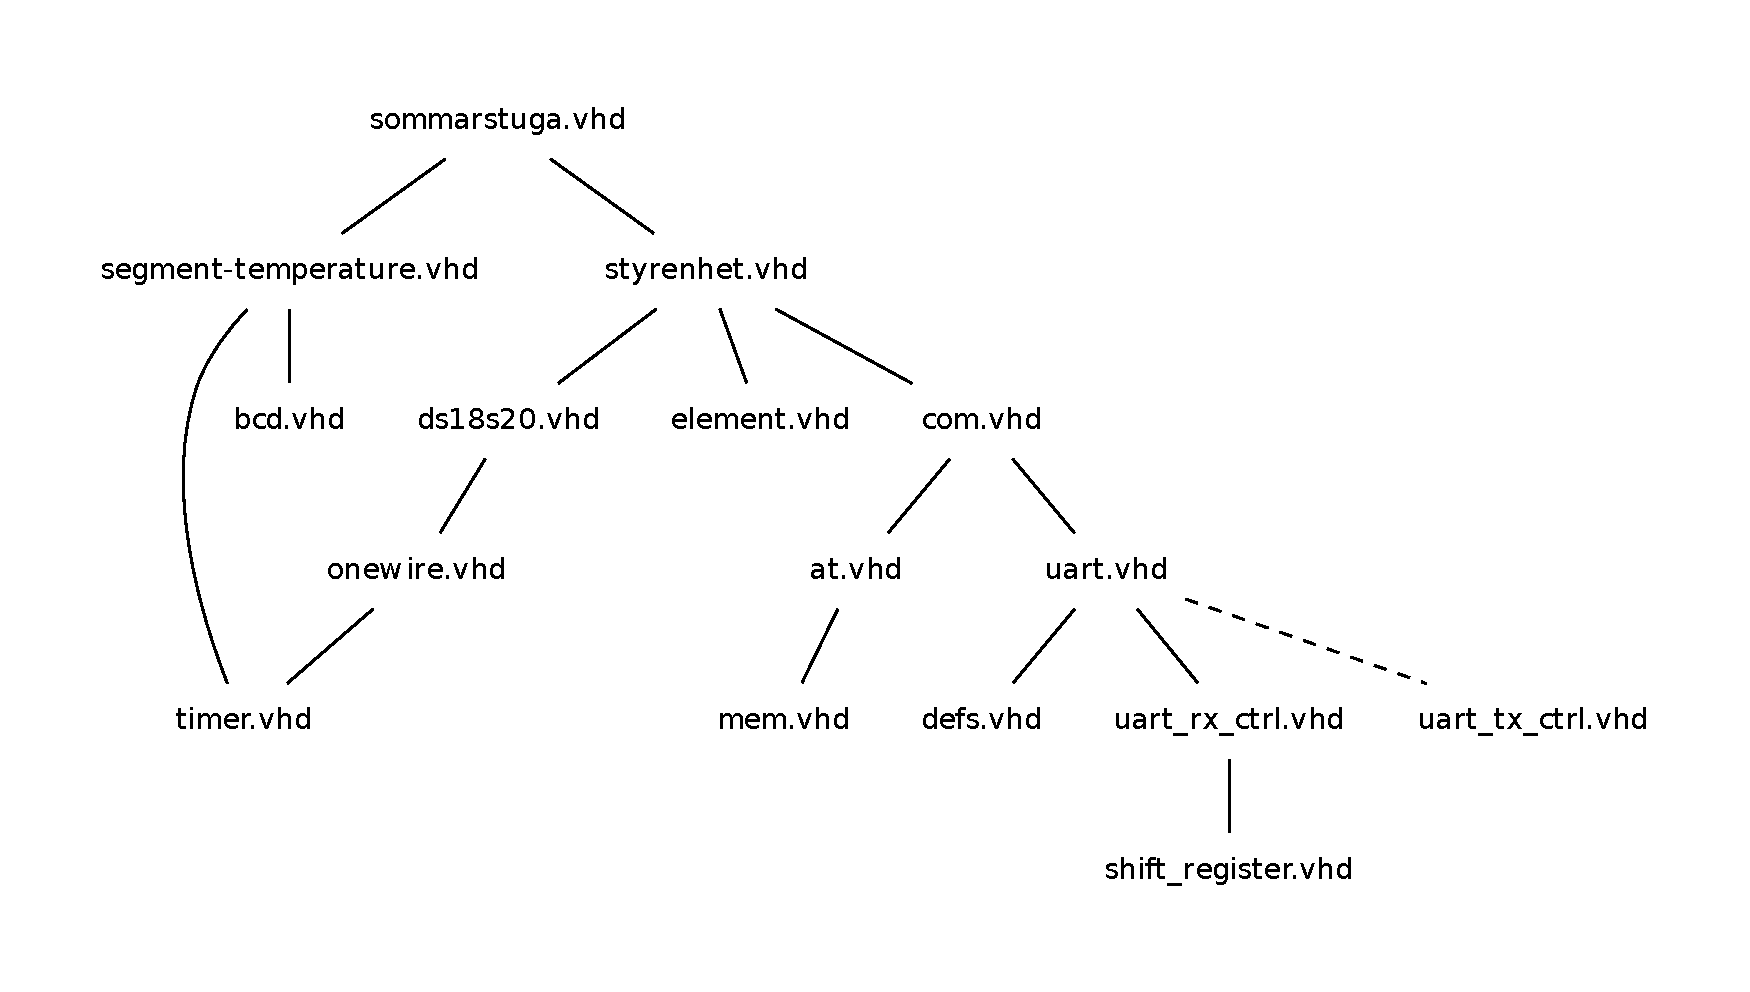
\includegraphics[width=\textwidth]{filstruktur.pdf}
\caption{Övergripande bild hur VHDL-moduler relaterar till varandra. Observera att uart\_tx\_ctrl.vhd ej är egenproducerad.}
\end{figure}


%\newcommand{\vhdl}[1]{\clearpage\subsection{#1}\label{sec:code:#1}%\lstinputlisting{../#1}}
%\vhdl{onewire.vhd}
%\vhdl{ds1820.vhd}
%\vhdl{segment-temperature.vhd}
%\vhdl{timer.vhd}
%\vhdl{bcd.vhd}


\clearpage
\section{Arbetsredogörelse}

\subsection{Christian}
\begin{itemize}
\item Jag har gjort blockschemat, tagit fram hur databussarna ska se ut (bredden på dem), hur många som behövs och var de ska vara någonstans.
\item Skrivit koden för:
	\begin{itemize}
	\item Styrenheten.
	\item Hantering utav elementen.
	\item Översta lagret av delblocket Kommunikation.
	\end{itemize}
\item Jag lödde fast den ytmonterade temperatursensorn, som sen visade sig vara fel krets.
\item Jag har satt ihop själva grundstrukturen för denna rapport och skrivit flertalet av kapitlen.
\item Varit med och löst problemet med UART-mottagaren, beträffande när inkommande data ska börja att samplas för att kunna avgöra huruvida en bit är 1 eller 0  och hur länge datan ska samplas för att göra avgörandet.
\item Tagit fram strukturen för hur AT-kommandona ska hanteras. Hur gsm-modulen förmedlar att ett nytt sms inkommit och hur innehållet i sms:et sedan hämtas ut ur gsm-modulens minne.
\item Jag har skapat pinlayouten samt ritat kretsschemat, med hjälp av ett CAD program. Både pinlayouten och kretsschemat finns i appendix. Har även skapat signallistan för styrenheten och elementen.
\end{itemize}


\subsection{Christoffer Öjeling}
\begin{itemize}
	\item Alla Komponenter för mätning och avläsning av temperatur från DS18S20 inkluside hjälpfunktioner.
	\item Lött den korrekta DS18S20-konstruktionen på ett mönsterkort.
	\item Visning av ett binärt tal på FPGAns 7-segmentsdisplay.
	\item Testning och verifikation av DS18S20 kontrollen.
	\item Binär till BCD konverterare.
	\item Allt i rapporten som relaterar till temperatursensorn DS18S20 och 7-segmentsdisplayn.
	\item Följande VHDL-moduler:
	\begin{itemize}
%		\item \fullref{sec:code:onewire.vhd}
%		\item \fullref{sec:code:ds1820.vhd}
%		\item \fullref{sec:code:segment-temperature.vhd}
%		\item \fullref{sec:code:timer.vhd}
%		\item \fullref{sec:code:bcd.vhd}
		\item onewire.vhd
		\item ds18s20.vhd
		\item segment-temperature.vhd
		\item timer.vhd
		\item bcd.vhd
	\end{itemize}
\end{itemize}

\subsection{Jan}
\begin{itemize}
	\item Kommunikationsmodul implementering
	\item UART modul
	\item AT modul
	\item Avkodning / kodning av AT-kommando
	\item Allt i rapporten som relaterar till kommunikationsmodulen.
	\item Följande kodfiler
		\begin{itemize}
		\item Defs.vhd
		\item Uart.vhd
		\item At.vhd
		\item Mem.vhd
		\item Shift\_register.vhd
		\item Uart\_rx\_ctrl.vhd
		\end{itemize}
\end{itemize}



\end{document}
